\documentclass[11pt]{article}
\usepackage{styletemplate}

\setlength{\parindent}{0pt}
\begin{document}

\title{\textbf{Quantum Grothendieck Polynomials for Partial Flags}}
\author{David Yang \and Zoe Markman}
\date{Summer 2024}

\maketitle

\section{Background Material}
\subsection{Schubert Polynomials}

Begin with the longest permutation in $S_n$, $w_0 = n \, n-1 \, \dots 1$. The Schubert polynomial for $w_0$ is
\[
    \mathfrak{S}_{w_0}(x) = x_1^{n-1} x_2^{n-2} \dots x_{n-1}.
\]

\begin{definition}[Divided Difference Operator]
The \textit{divided difference operator}, defined on the polynomial ring $\Z[x_1, \dots, x_m]$, is
\[
    \delta_i(f) = \frac{f - s_i(P)}{x_i - x_{i+1}}
\] 
where $s_i(f)$ is the result of interchanging $x_i$ and $x_{i+1}$ in $f$, a polynomial in $\Z[x_1, \dots, x_m]$, for any $i$ between $1$ and $m-1$.
\end{definition}

\begin{definition}[Schubert Polynomials]
The \textbf{Schubert polynomial} corresponding to $w \in S_n$ can be found recursively from $\mathfrak{S}_{w_0}$ by the rule
\[
    \mathfrak{S}_{ws_i} = \delta_i(\mathfrak{S}_w) \text{ if $w(i) > w(i+1)$}.
\]
\end{definition}


When we refer to the complete flag manifold $Fl(1,2,3,4)$, the Schubert polynomials corresponding to the permutations in $S_4$ form the basis for the cohomology ring of the flag manifold.
\[
    Fl(1, 2, 3, 4) \leftrightarrow S_4
\]
In general, for a given flag manifold $Fl(d_1, d_2, \dots, d_k)$ with $d_k = n$ we find that the basis for the cohomology corresponds to a subset of the Schubert polynomials of $S_n$:
\[
    Fl(d_1, d_2, \dots, d_k) \leftrightarrow \{\mathfrak{S}_w \in S_n \mid w \text{ has descents } \subseteq \{ d_1, d_2, \dots, n\} \}
\]

Take the specific case of $Gr(2, 4) = Fl(2, 4)$. The basis corresponds to Schubert polynomials of permutations $w \in S_4 \mid w \text{ has descent possibly at $2$}$; the permutations in said basis are Schubert polynomials for $[1\, 2 \mid 3 \,4]$, $[1\,3 \mid 2\,4]$, $[1\, 3 \mid 2\,4]$, $[1\,4 \mid 2\,3]$, $[2\,3 \mid 1\,4]$, $[2\,4 \mid 1\,3]$, and $[3\,4 \mid 1\,2]$. \\

There is an association between the Schubert polynomials corresponding to each of these permutations and an associated Schur polynomial, characterized by the following rule: let $w = w_1 w_2 \dots w_n$. 
\begin{quote}
\textit{If $w_i < w_{i+1}$ for all $i \neq r$ (i.e. there is just one descent at index $r$), $\mathfrak{S}_w$ is the Schur polynomial $s_\lambda(x_1, \dots, x_r)$, where $\lambda = (w_r - r, \dots, w_2 - 2, w_1 - 1)$.}
\end{quote}

The above rule is extremely useful for identifying Schuberts as Schurs. For example, consider the Schubert polynomial corresponding to the permutation $[2\,4 \mid 1\,3]$. There is a descent at index $2$, and so $\lambda = (w_2 - 2, w_1 - 1) = (4 - 2, 2 - 1) = (2, 1)$ and
\[
    \mathfrak{S}_{[2\,4 \mid 1\,3]} = s_{(2, 1)}(x_1, x_2).
\]

The same rule applies for other permutations with one descent. For example, 
\[
    \mathfrak{S}_{[2 \mid 1\,3\,4]} = s_{(1)}(x_1).
\]
In particular, the rule also helps us realize that all Schur polynomials (of a finite number of variables) are Schubert polynomials; any Schur can be reconciled with a given permutation with one descent, which corresponds to a Schubert polynomial. \\

\textit{Additional Info: Schubert polynomials can be realized through pipe dreams or rc-graphs -- see \href{https://sites.math.washington.edu/~billey/papers/bjs.pdf}{Billey-Jockusch-Stanley} for more information.}

\subsection{Bases and Quantum Cohomology in Full Flag $Fl_n$}

As we have just seen, one basis for the cohomology ring $H^* Fl_n$ is the set of Schubert polynomials corresponding to each permutation in $S_n$, or
\[
    \{ \mathfrak{S}_w(x_1, \dots, x_n) \mid w \in S_n \}.
\]

The set of Schubert polynomials is a positive basis; indeed, the Littlewood-Richardson Rule for Schur polynomials generalizes to Schuberts, and we have
\[
    \mathfrak{S}_u \mathfrak{S}_v = \sum_{w} c_{uv}^w \mathfrak{S}_w
\]
where each $c_{uv}^w$ is a unique (because the Schuberts are a basis) nonnegative coefficient. \\

Another well-known basis is known as the \textbf{\textit{standard elementary monomials}}, of the form
\[
    \{e_{i_1}(1) \cdots e_{i_{n-1}}(n-1) \mid 0 \leq i_k \leq k \}
\]
where each $e_k(p)$ corresponds to the elementary symmetric polynomial of degree $k$ in $p$ variables $x_1, \dots, x_p$. Contrary to the previous Schubert basis, this is not a positive basis. For example, consider $Fl(3)$ and the product $e_1(1) \cdot e_1(1).$ We have that
\begin{align*}
    e_1(1) \cdot e_1(1) &= x_1^2 \\
    &= x_1(x_1 + x_2) - x_1x_2 \\
    &= e_1(1)e_1(2) - e_2(2).
\end{align*}

Note that each of these bases has precisely $n!$ entries, a defining characteristic for the bases of a complete flag manifold. 

The quantized standard elementary monomials in both full and partial flag manifolds can be realized from two different methods. We begin with a discussion of the quantized standard elementary monomials in the full flag case. From Fomin-Gelfand-Postnikov (FGP), we can realize the quantized standard elementary monomial through the characteristic polynomial of the matrix
\[
    G_n = \begin{bmatrix}
    x_1 & q_1 & 0 & \dots & 0 \\
    -1 & x_2 & q_2 & \dots & 0 \\
    \vdots & \vdots & \vdots & \ddots & \cdots \\
    0 & 0 & 0 & \dots & x_n
    \end{bmatrix},
\]
which is constructed with the $x_i$ terms on the main diagonal, the quantum $q$ terms on the superdiagonal, $-1$ terms on the subdiagonal, and $0$'s elsewhere. \\

With the property
\[
    \det(1 + \lambda G_n) = \sum\limits_{i=0}^n E_i(n) \lambda^i,
\]
we realize the quantized standard elementary monomial $E_{i-j}(n)$ as the coefficient of the $\lambda^j$ term in $\det(1 + \lambda G_n)$. \\

\begin{eg}[Matrix Approach for Quantized Monomials in $Fl_3$]

We will begin by using the matrix approach. Note that
\[
    G_3 = \begin{bmatrix}
    x_1 & q_1 & 0 \\
    -1 & x_2 & q_2 \\
    0 & -1 & x_3
    \end{bmatrix}.
\]
We see that $1 + \lambda G_3 = \begin{bmatrix}
    1 + \lambda x_1 & \lambda q_1 & 0 \\
    -\lambda & 1 + \lambda x_2 & \lambda q_2 \\
    0 & -\lambda & 1 + \lambda x_3
    \end{bmatrix}$
so $\det (1 + \lambda G_1)$ is the determinant of the upper left $1 \times 1$ corner of $G_3$, $\det (1 + \lambda G_2)$  is the determinant of the upper left $2 \times 2$ corner of $G_3$, and $\det (1 + \lambda G_3)$ is the determinant of the whole matrix. We get

\[
    \det (1 + \lambda G_1) = 1 + \lambda x_1,
\]
\begin{align*}
    \det (1 + \lambda G_2) &= (1+\lambda x_1)(1+\lambda x_2) + \lambda^2 q_1 \\
    &= 1 + \lambda (x_1 + x_2) + \lambda^2 (x_1x_2 + q_1).
\end{align*}

Recognizing the quantum standard elementary monomials as the coefficients of the respective determinants, we get that
\[
    \boxed{E_1(1) = x_1, E_1(2) = x_1 + x_2, \text{ and } E_2(2) = x_1x_2 + q_1}.
\]
\end{eg}

\vspace{0.5cm}
Alternatively, one can recognize the standard elementary monomials through the use of Dynkin diagrams. Consider some flag manifold $Fl(d_1, \dots, d_n)$; by convention, $d_0 = 0$. The number of quantum terms $q_i$ corresponds to the number of steps in the flag, which is $n-1$. For each quantum term $q_i$ from $i = 1$ to $n-1$, $q_i$ covers $x_{d_{i-1} + 1}$ to $x_{d_{i+1}}$. \\

The \textit{\textbf{Dynkin diagram}} represents the relationships between the $x$ and $q$ terms, and can be used to determine the quantized standard elementary monomials. \\

In general, recall that the standard elementary monomial $e_i(j)$ represents the sum of monomials of degree $i$ from the set $\{x_1, \dots, x_j\}$ that cover each $x_i$ at most once. \\

Similarly, the \textit{quantized standard elementary monomial} $E_i(j)$ represents the sum of monomials of degree $i$ from the set $\{x_1, \dots, x_j\}$ and corresponding $q$ entries that cover each $x_i$ at most once. \\

\begin{eg}[Dynkin Example in $Fl(1, 2, 4)$]
Consider the following Dynkin diagram corresponding to the flag manifold $Fl(1, 3, 4)$ -- $q_1$ spans $x_{d_0 + 1} = x_1$ to $x_{d_1} = 3$ and $q_2$ spans $x_{d_1 + 1} = x_2$ to $x_{d_2} = x_4$. 
\begin{center}
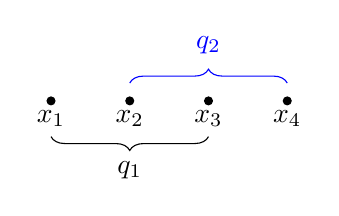
\begin{tikzpicture}
\filldraw[black] (0, 0) circle (0.05);
\filldraw[black] (1, 0) circle (0.05);
\filldraw[black] (2, 0) circle (0.05);
\filldraw[black] (3, 0) circle (0.05);
\draw [decorate,decoration={brace,amplitude=5pt,mirror,raise=3ex}]
  (0,0) -- (2,0) node[midway,yshift=-2.5em]{$q_1$};
  \draw [decorate,decoration={brace,amplitude=5pt,raise=1.5ex},color={blue}]
  (1,0) -- (3,0) node[midway,yshift=2em]{$q_2$};
\node[below] at (0, 0) {$x_1$};
\node[below] at (1, 0) {$x_2$};
\node[below] at (2, 0) {$x_3$};
\node[below] at (3, 0) {$x_4$};  
\end{tikzpicture}
\end{center}

We have that
\[
    e_4(4) = x_1x_2x_3x_4 + q_1x_4 + x_1q_2.
\]
\end{eg}

\begin{eg}[Dynkin Approach for Quantized Monomials in $Fl_3$]
The Dynkin Diagram for $Fl_3$ is as follows:
\begin{center}
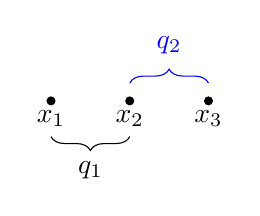
\begin{tikzpicture}
\filldraw[black] (0, 0) circle (0.05);
\filldraw[black] (1, 0) circle (0.05);
\filldraw[black] (2, 0) circle (0.05);
\draw [decorate,decoration={brace,amplitude=5pt,mirror,raise=3ex}]
  (0,0) -- (1,0) node[midway,yshift=-2.5em]{$q_1$};
  \draw [decorate,decoration={brace,amplitude=5pt,raise=1.5ex},color={blue}]
  (1,0) -- (2,0) node[midway,yshift=2em]{$q_2$};
\node[below] at (0, 0) {$x_1$};
\node[below] at (1, 0) {$x_2$};
\node[below] at (2, 0) {$x_3$};
\end{tikzpicture}
\end{center}
We can easily identify the corresponding quantized standard elementary monomials:
\[
    \boxed{E_1(1) = x_1, E_1(2) = x_1 + x_2, E_2(2) = x_1x_2 + q_1},
\]
which match the matrix approach calculations.
\end{eg}

\begin{remark}
The above two approaches are equivalent formulations for determining the quantized standard elementary monomials. The diagram approach can be generalized to partial flag manifolds as is, whereas the matrix approach has a similar but slightly more complicated structure in the partial flag case.
\end{remark}

\subsection{Quantum Schubert Polynomials}
\textbf{\textit{Quantum Schubert polynomials}} arise as ``quantized'' versions of the Schubert polynomials. Consider the Schubert polynomial $\mathfrak{S}_{[3 \, 1 \, 2]}$ in $S_3$. One can find, using the divided difference operator, that $\mathfrak{S}_{[3 \, 1 \, 2]} = x_1^2$ -- from the above example, we know that this can also be rewritten in the standard elementary monomial basis:
\begin{align*}
    \mathfrak{S}_{[3 \, 1 \, 2]} &= x_1^2 \\
    &= e_1(1) e_1(2) - e_2(2).
\end{align*}

To determine the corresponding quantum Schubert polynomial, we simply replace each of the standard elementary monomials with their quantized versions (represented by capital letters), so

\begin{align*}
    \mathfrak{S}_{[3 \, 1 \, 2]}^q &= E_1(1) E_1(2) - E_2(2) \\
    &= x_1(x_1 + x_2) - (x_1x_2 + q_1) \\
    &= x_1^2 - q_1
\end{align*}

The quantum Schubert polynomials serve as a basis for the quantum cohomology of $Fl(3)$. As we saw in the cohomology case, in general, the basis for the quantum cohomology of a partial flag $Fl(d_1, d_2, \dots, d_k)$ $ \leftrightarrow \{\mathfrak{S}_w \in S_n \mid w \text{ has descents } \subseteq \{ d_1, d_2, \dots, d_k\} \}$. \\

The following is a Quantum Monk rule for products of Quantum Schuberts in Complete Flags:
\begin{theorem*}[Quantum Monk for Quantum Schubert in Complete Flags, FGP (584)]
Let $t_{ab}$ be the transposition of positions $a$ and $b$.
    \[
        \mathfrak{S}_{s_r}^q \mathfrak{S}_{w}^q = \sum \mathfrak{S}_{wt_{ab}}^q + \sum q_{cd}\mathfrak{S}_{wt_{cd}}^q
    \]
    where the first sum is over $a \leq r < b$ such that $l(wt_{ab}) = l(w) + 1$ and the second sum is over $c \leq r < d$ such that $l(wt_{cd}) = l(w) - l(t_{cd}) = l(w) - 2(d - c) + 1$. \textit{note: $q_{cd} = q_c q_{c+1} \dots q_{d-1}$.}
\end{theorem*}


\subsection{Grothendieck Polynomials}

Begin with the longest permutation in $S_n$, $w_0 = n \, n-1 \, \dots 1$. The Grothendieck polynomial of $w_0$ is the same as the Schubert polynomial for $w_0$:
\[
    \mathfrak{G}_{w_0}(x) = x_1^{n-1} x_2^{n-2} \dots x_{n-1}.
\]
\begin{definition}[Grothendieck Polynomials]
Let $\delta_i = \frac{f - s_i(f)}{x_i - x_{i+1}}$ be the divided difference operator, and let $\pi_i = \delta_i(1-x_{i+1})$. 

The Grothendieck polynomials for $w \in S_n$ are defined as
\begin{align*}
    \mathfrak{G}_w(x_1, x_2, \ldots, x_n) &= \pi_{w^{-1}w_0}(x_1^{n-1} x_2^{n-2} \ldots x_{n-1}) 
\end{align*}
\end{definition}


\begin{definition}[Equivalent Formulations of Grothendiecks]
The \textit{isobaric divided difference operator} is defined as
\[
    \overline{\delta}_i(f) = \delta_i[(1-x_{i+1})f]
\] 
and the \textbf{Grothendieck polynomial} corresponding to $w \in S_n$ can be found recursively from $\mathfrak{G}_{w_0}$ by the rule
\[
    \mathfrak{G}_{ws_i} = \overline{\delta}_i(\mathfrak{G}_w) \text{ if $w(i) > w(i+1)$}
\]
\end{definition}

Some code on computing Grothendieck polynomials in Sage: \href{https://wiki.sagemath.org/combinat/MultivariatePolynomials}{how to compute these in sage}!

Note that the lowest degree homogenous part of $\mathfrak{G}_w$ is given by $\mathfrak{S}_w$ (the corresponding Schubert polynomial). 

\begin{theorem}[Grothendieck Pieri, from Lenart and Maeno]
    \begin{equation*}
        \mathfrak{G}_wg_p^k = \sum_\gamma m_p(\gamma) \mathfrak{G}_{\text{end}(\gamma)}
    \end{equation*} 
    where the sum is over all $k$-Pieri chain $\gamma$ on the infinite symmetric group that begin at $w$.

    We define $g_p^k = \mathfrak{G}_{c[k,p]} = \sum_{i=p}^k (-1)^{i-p} {{i-1}\choose{p-1}} e_i^k$. We let $\gamma$ denote a $k$-Pieri chain (see definition 2.14), $m_p(\gamma) = (-1)^{l(\gamma) -p}$ times the number of $p$-markings of $\gamma$.
\end{theorem}
The $k$-Pieri chain looks complicated — The monk formula covers the case when $p = 1$, and seems much nicer. I think the $k$-Pieri chain is the big (gross) thing that lets you generalize.

\begin{definition}[Quantum Grothendieck Polynomials]
    The \textbf{Quantum Grothendieck polynomial} $\mathfrak{G}_w^q$, for $w \in S_n$, is
    \begin{equation*}
        \mathfrak{G}_w^q = \hat{Q}(\mathfrak{G}_w) \in \Z[q,x]
    \end{equation*}
\end{definition}
The quantum Grothendiecks for $S_3$ are in example 3.19 of Lenart-Maeno, and a combinatorial formula is given later in the paper. \\

\begin{theorem}[Quantum Monk for Grothendieck -- Theorem 6.4 in LeM]

We have
\begin{equation*}
    \G_w^q \G_{s_k}^q = \sum_\pi (-1)^{l(\pi)- 1}q(\pi) \G_{end(\pi)} ; 
\end{equation*}
the summation is over all nonempty paths $\pi$ in the quantum $k$-Bruhat graph (of $S^\infty$) of the form 
\begin{equation*}
    w = w_0 \rightarrow w_1 \rightarrow \ldots \rightarrow w_s = \text{end}(\pi)
\end{equation*}
where $(a_1, b_1) \prec (a_2,b_2) \prec \ldots \prec (a_s,b_s)$.
\end{theorem}

For calculations with quantum Grothendiecks, there is the following \href{https://ow3.math.rutgers.edu/~asbuch/equivcalc/}{Maple Package for Quantum Grothendiecks}.

\newpage

\begin{table}[!h]
\centering
\caption{Grothendiecks for $S^3$}
\begin{tabular}{|p{2cm}|c|p{10cm}|}
\hline
Permutation &  Grothendieck  &  Quantum Grothendieck  \\ \hline
123 & 1 & 1 \\ \hline
132 & $-x_1x_2 + x_1 + x_2$ & $x_1x_2q_2 - x_1x_2 - x_1q_2 - x_2q_2 + x_1 + x_2 + q_2$ \\ \hline
213 & $x_1$ & $-x_1q_1 + x_1 + q_1$ \\ \hline
231 & $x_1x_2$ & $-x_1x_2q_2 + x_1x_2 - x_1q_1 + x_1q_2 + q_1$ \\ \hline
312 & $x_1^2$ & $
    x_1^2q_1^2 + x_1x_2q_1q_2  - 2x_1^2q_1 - x_1x_2q_1 - 2x_1q_1^2 - x_1q_1q_2 
    - x_2q_1q_2 + x_1^2 + 3x_1q_1 + x_2q_1 + q_1^2 + q_1q_2 - q_1$ \\ \hline 
321 & $x_1^2x_2$ & $x_1^2x_2q_1q_2 - x_1^2x_2q_1 + x_1^2q_1^2 - x_1^2x_2q_2 - x_1^2q_1q_2 - x_1x_2q_1q_2 + x_1^2x_2 - x_1^2q_1 + x_1x_2q_1 - 2x_1q_1^2 + x_1^2q_2 + x_1q_1q_2 + x_1q_1 + q_1^2$ \\ \hline 
\end{tabular}
\end{table}

\end{document}
